\section{Metrics}
\label{sec:evaluation:metrics}

We breakdown the evaluation of our pipeline mapped its four stages=: (1) bib detection, (2) text detection within a bib crop, (3) \gls{ocr} within a single bib crop against the ground truth, (4) overall performance on an entire image.

\subsection{Bib Detection Performance}
\label{sec:evaluation:metrics:bib}

% Talk about Model Peformance Measure
% Confidence Measure
% Precision, Recall, F-Score

In addition to the standard precision, recall and \fscore{} metrics defined in \cref{sec:background:metrics}, we develop a secondary measure for our model performance based on the number of bib detections made in an image. For the ideal case, we assess the bib's detection accuracy assuming a binary scenario (the pipeline either finds the bib or it does not) and, where more than one detection is made, we limit its performance to 1. For the realistic case, the bib detection model performance is assessed as the number of estimated bibs found in the image divided by the total number of ground truth bibs. Thus, the resulting performance metric is in the range $[0, 1]$.

This means that, regardless of the number of bibs that are identified, as long as the number of estimated bibs is equal to or greater than the number of ground truth bibs, it is identified as a hit. Any more identified bibs are either classified as false positive estimates, or cases that were not considered for ground truth annotation.

Thus, given a set of ground truth bibs, $T_{bib}$, and estimates $E_{bib}$, we define the addition metric of bib performance, $p_{bib}$, as:
\begin{align*}
  p_{bib} =
  \begin{cases}
    0,                                          & \textrm{if}\ \lvert\,T_{bib}\,\rvert = 0\\
    \min\left(1, \frac{\lvert\,E_{bib}\,\rvert}{\lvert\,T_{bib}\,\rvert}\right), & \textrm{otherwise}
  \end{cases}
\end{align*}

\noindent
Therefore, this performance metric captures \textit{at least} all valid and correct bibs in the image, while ignoring the false alarms. As this stage, the metric is only dealing with bib \textit{detection}. Our primary concern is with regards to \textit{detecting} and not \textit{recognising} bibs: having false positives detected in this stage is not an issue as we are likely to eliminate them in further stages should the estimated region not be a bib at all, thus maintaining our overall performance (\cref{sec:evaluation:metrics:overall}).

\subsection{Text Detection Performance}

For text and character detection, we follow a similar process to that outlined in \cref{sec:evaluation:metrics:bib}. Text detection works in a binarised matter: within a bib crop, the text detection model either accurately detects the ground truth \gls{rbn} region, or it does not. For character segmentations, Tesseract's \gls{lstm} network either accurately detects all or partially detects characters within the \gls{rbn}. The metric focus here is, once again, a partial match to ensure that \textit{at least} all matches that can be made are made, and anything more is ignored.

\subsection{Character Recognition}

Character recognition introduces two additional metrics. For a \textit{single} \gls{rbn}, we define the recognition performance as the number of characters that match the characters within the ground truth \gls{rbn}. Given a set of ground truth \gls{rbn} sequences in an image, $T_{rbn}$, and recognition estimations made, $E_{rbn}$, a single element (either a ground truth or estimated \gls{rbn}) in either set is defined as $t$ and $e$, respectively.

Given that an \gls{rbn} is a set of characters, $t$ and $e$ are therefore sets of characters, and thus, the character recognition performance on a single \gls{rbn}, $p_{rbn}$ is measured as:
\begin{align*}
  p_{rbn} = \left\{ \max \left(0.5 \times \left(\frac{\lvert\,e\,\cap\,t\,\rvert}{\lvert\,e\,\rvert} + \frac{\lvert\,e\,\cap\,t\,\rvert}{\lvert\,t\,\rvert} \right) \right)\ |\ \forall e \in E, \forall t \in T \right\}
\end{align*}

\subsection{Overall Performance}
\label{sec:evaluation:metrics:overall}

We represent our pipeline as a way to narrow in on an image toward the true positive bib numbers that exist. Represented in set notation, the ground truth is a set of \gls{rbn} sequences within the image, $T_{rbn}$, and our estimations of those \glspl{rbn} are another set, $E_{rbn}$. Therefore, we formally describe that true positive matches are all estimations that fall within the ground truth ($E_{rbn} = T_{rbn}$, $E_{rbn} \subset T_{rbn}$), and all false positives are introduced when this is not the case ($T_{rbn} \subset E_{rbn}$, $E_{rbn} \not\subset T_{rbn}$,  $E_{rbn} \cap T_{rbn} = \varnothing$).

Represented as Euler diagrams (\cref{fig:evaluation:metrics:character_rec:sets}), we visualise and describe such cases with context. Initially, our pipeline starts with \cref{fig:evaluation:metrics:character_rec:sets:problematic}---we narrow down our estimations using person, bib and text detection to eliminate false positives (that penalise the overall performance due to invalid recognitions), bringing us closer towards the ground truth.

If our pipeline is successful, we either end up with \cref{fig:evaluation:metrics:character_rec:sets:good}, or better, \cref{fig:evaluation:metrics:character_rec:sets:best}. With the former, we have recognised all \glspl{rbn} that are within the ground truth, though are still some false negatives. Thus our estimation set is not complete, unlike \cref{fig:evaluation:metrics:character_rec:sets:best} where the estimation set matches the ground truth exactly. We consider \cref{fig:evaluation:metrics:character_rec:sets:good} as `good' because, while it does not detect every \gls{rbn}, we do not introduce false positives that do not exist in the image and introduce false data.

If our pipeline is not successful, we end up with \cref{fig:evaluation:metrics:character_rec:sets:moderate,fig:evaluation:metrics:character_rec:sets:problematic,fig:evaluation:metrics:character_rec:sets:worst}. In  \cref{fig:evaluation:metrics:character_rec:sets:moderate}, we see that---while the ground truths are within the subset of estimations---we produce false positives, and therefore mis-informed data that penalises performance. Similarly, in \cref{fig:evaluation:metrics:character_rec:sets:problematic}, there are still false positives, but---problematically---also false negatives as we are not recognising ground truth. (This must be penalised further as we introduce incorrect data and do not \textit{fully} report correct data.) Lastly, when the ground truth and estimations are mutually exclusive (\cref{fig:evaluation:metrics:character_rec:sets:worst}), the pipeline \textit{only} reports false positives.

\begin{figure}[p]
  \centering
  \hspace{\fill}
  \begin{subfigure}[b]{0.475\textwidth}
    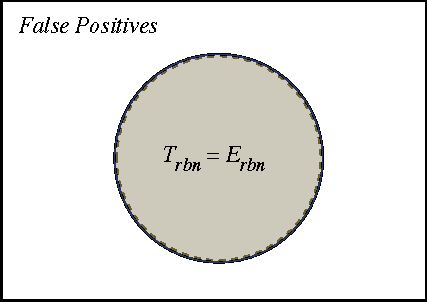
\includegraphics[width=\textwidth]{images/evaluation/set_explain/T_is_E}
    \caption{Best performance as $E_{rbn} = T_{rbn}$.}
    \label{fig:evaluation:metrics:character_rec:sets:best}
  \end{subfigure}
  \hspace{\fill}
  \begin{subfigure}[b]{0.475\textwidth}
    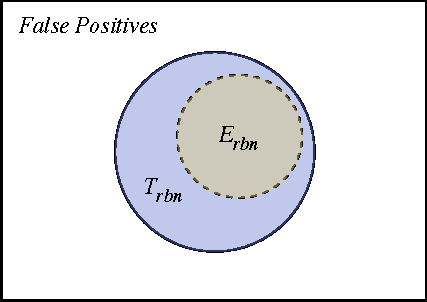
\includegraphics[width=\textwidth]{images/evaluation/set_explain/E_subset_of_T}
    \caption{Good performance as $E_{rbn} \subset T_{rbn}$.}
    \label{fig:evaluation:metrics:character_rec:sets:good}
  \end{subfigure}
  \hspace{\fill}
  \\
  \bigskip
  \hspace{\fill}
  \begin{subfigure}[b]{0.475\textwidth}
    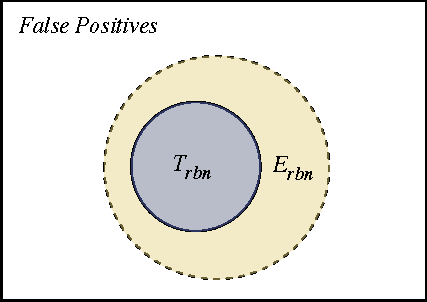
\includegraphics[width=\textwidth]{images/evaluation/set_explain/T_subset_of_E}
    \caption{Moderate performance as $T_{rbn} \subset E_{rbn}$.}
    \label{fig:evaluation:metrics:character_rec:sets:moderate}
  \end{subfigure}
  \hspace{\fill}
  \begin{subfigure}[b]{0.475\textwidth}
    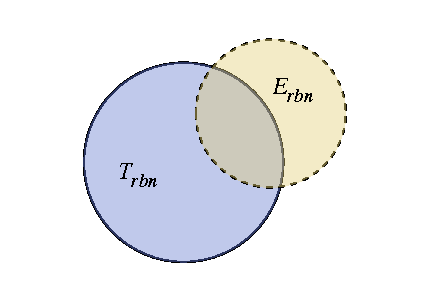
\includegraphics[width=\textwidth]{images/evaluation/set_explain/E_not_subset_of_T}
    \caption{Problematic performance as $T_{rbn} \not\subset E_{rbn}$.}
    \label{fig:evaluation:metrics:character_rec:sets:problematic}
  \end{subfigure}
  \hspace{\fill} 
  \bigskip
  \\
  \begin{subfigure}[b]{0.475\textwidth}
    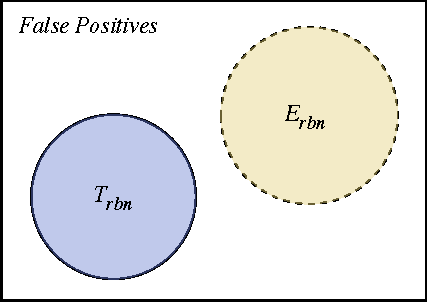
\includegraphics[width=\textwidth]{images/evaluation/set_explain/T_mutually_exclusive_E}
    \caption{Worst performance as $E_{rbn} \cap T_{rbn} = \varnothing$.}
    \label{fig:evaluation:metrics:character_rec:sets:worst}
  \end{subfigure}
  \bigskip
  \\
  \caption[Euler diagram to illustrate OCR performance]{Various scenarios of \gls{ocr} performance. The order of subfigures indicate the degrading performance. Subfigures \subref{fig:evaluation:metrics:character_rec:sets:best} and \subref{fig:evaluation:metrics:character_rec:sets:good} show the successful cases, while non-successful cases are shown in \subref{fig:evaluation:metrics:character_rec:sets:moderate} to \subref{fig:evaluation:metrics:character_rec:sets:worst}. }
  \label{fig:evaluation:metrics:character_rec:sets}
\end{figure}